\section{Cropflip}

\subsection{Descripción}
La imagen destino del filtro consiste en invertir verticalmente (flip) un recorte (crop) de la imagen fuente a partir de offsets dados como parámetro. El ancho y alto en píxeles de la imagen destino también se pasa como parámetros.
La descripción matemática está dada por la fórmula:

$$ O_{i,\ j}^{k}=I_{tamy+offsety-i-1, \ \ offsetx+j}^{k} $$

Donde el 'crop' de la imagen input corresponde con los píxeles del tipo:

$$
I_{offsety+i, \ \ offsetx+j}^{k} 
\qquad \text{con} \quad 0 \leq i < tamy \ \ \ 0 \leq j < tamx 
$$

\begin{table}[h]
\centering
\mem
\begin{tabular}{l|c|c|c|c|c|c|l}
 & \multicolumn{1}{l|}{}      & \multicolumn{1}{l|}{}       & \multicolumn{1}{l|}{}       & \multicolumn{1}{l|}{}       & \multicolumn{1}{l|}{}       & \multicolumn{1}{l|}{}      &  \\ \hline
 & \cellcolor[HTML]{FFCB2F}$I_{30}$ & \cellcolor[HTML]{FFCB2F}$I_{31}$  & \cellcolor[HTML]{FD6864}$I_{32}$  & \cellcolor[HTML]{FD6864}$I_{33}$  & \cellcolor[HTML]{FD6864}$I_{34}$  & \cellcolor[HTML]{FD6864}$I_{35}$ &  \\ \hline
 & \cellcolor[HTML]{FFCB2F}$I_{24}$ & \cellcolor[HTML]{FFCB2F}$I_{25}$  & \cellcolor[HTML]{FD6864}$I_{26}$  & \cellcolor[HTML]{FD6864}$I_{27}$  & \cellcolor[HTML]{FD6864}$I_{28}$  & \cellcolor[HTML]{FD6864}$I_{29}$ &  \\ \hline
 & \cellcolor[HTML]{FFCB2F}$I_{18}$ & \cellcolor[HTML]{FFCB2F}$I_{19}$ & \cellcolor[HTML]{FD6864}$I_{20}$ & \cellcolor[HTML]{FD6864}$I_{21}$ & \cellcolor[HTML]{FD6864}$I_{22}$  & \cellcolor[HTML]{FD6864}$I_{23}$ &  \\ \hline
 & \cellcolor[HTML]{FFCB2F}$I_{12}$ & \cellcolor[HTML]{FFCB2F}$I_{13}$ & \cellcolor[HTML]{FD6864}$I_{14}$ & \cellcolor[HTML]{FD6864}$I_{15}$ & \cellcolor[HTML]{FD6864}$I_{16}$  & \cellcolor[HTML]{FD6864}$I_{17}$ &  \\ \hline
 & \cellcolor[HTML]{FFCB2F}$I_{6}$ & \cellcolor[HTML]{FFCB2F}$I_{7}$ & \cellcolor[HTML]{FFCB2F}$I_{8}$ & \cellcolor[HTML]{FFCB2F}$I_{9}$ & \cellcolor[HTML]{FFCB2F}$I_{10}$  & \cellcolor[HTML]{FFCB2F}$I_{11}$ &  \\ \hline
 & \cellcolor[HTML]{FFCB2F}$I_{0}$ & \cellcolor[HTML]{FFCB2F}$I_{1}$ & \cellcolor[HTML]{FFCB2F}$I_{2}$ & \cellcolor[HTML]{FFCB2F}$I_{3}$ & \cellcolor[HTML]{FFCB2F}$I_{4}$  & \cellcolor[HTML]{FFCB2F}$I_{5}$ &  \\ \hline
 & \multicolumn{1}{l|}{}      & \multicolumn{1}{l|}{}       & \multicolumn{1}{l|}{}       & \multicolumn{1}{l|}{}       & \multicolumn{1}{l|}{}       & \multicolumn{1}{l|}{}      &
\end{tabular}
\caption{Ilustracion de la imagen fuente en memoria. En rojo los pixeles del crop \newline
(offsetx = 2, offsety = 2, tamx = 4, tamy = 4)}
\end{table}

\begin{table}[h]
\centering
\mem
\begin{tabular}{l|c|c|c|c|l}
& \multicolumn{1}{l|}{}       & \multicolumn{1}{l|}{}   & \multicolumn{1}{l|}{}     & \multicolumn{1}{l|}{}      &  \\ \hline
 & \cellcolor[HTML]{FD6864}$I_{14}$ & \cellcolor[HTML]{FD6864}$I_{15}$ & \cellcolor[HTML]{FD6864}$I_{16}$  & \cellcolor[HTML]{FD6864}$I_{17}$ &  \\ \hline
 & \cellcolor[HTML]{FD6864}$I_{20}$ & \cellcolor[HTML]{FD6864}$I_{21}$ & \cellcolor[HTML]{FD6864}$I_{22}$  & \cellcolor[HTML]{FD6864}$I_{23}$ &  \\ \hline 
 & \cellcolor[HTML]{FD6864}$I_{26}$  & \cellcolor[HTML]{FD6864}$I_{27}$  & \cellcolor[HTML]{FD6864}$I_{28}$  & \cellcolor[HTML]{FD6864}$I_{29}$ &  \\ \hline
  & \cellcolor[HTML]{FD6864}$I_{32}$ & \cellcolor[HTML]{FD6864}$I_{33}$  & \cellcolor[HTML]{FD6864}$I_{34}$  & \cellcolor[HTML]{FD6864}$I_{35}$ &  \\ \hline
  & \multicolumn{1}{l|}{}       & \multicolumn{1}{l|}{}  & \multicolumn{1}{l|}{}      & \multicolumn{1}{l|}{}      &
\end{tabular}
\caption{Ilustracion de la imagen destino en memoria}
\end{table}




No es dificil notar que las filas del crop en la fuente no constituyen una tira contigua de píxeles en memoria, si no que se encuentran distanciadas por el tamaño en bytes de offsetx lo que implica que necesitaremos iterar en dos ciclos anidados para poder procesar el crop.

\subsection{Implementaciones}
Al no involucrar operaciones aritméticas entre componentes de la imagen, las implementaciones del filtro se centran en accesos a memoria. Por lo tanto, las implementaciones solamente difieren en el modo en que se copian y asignan píxeles a la imagen output, radicando en esos métodos nuestro foco de análisis. 
\subsubsection{Implementaciones C y SSE}
La implementación C simplemente se trata de recorrer la imagen con una sola variable aplicando pixel a pixel la transformación dada por la fórmula matemática previamente mencionada. Mientras que la implementación corresponiente a SSE recorre la imagen fuente desde la fila superior del recuadro ($I_{32}$ en el cuadro 1) del crop hacia abajo de a 4 píxeles por iteración como indica el siguiente pseudo-código: 


\begin{codesnippet}
\begin{verbatim}

temp = src + offsetx*4 +srcRowSize*(offsety+tamy-1)       
{Apunta al primer píxel de la esquina superior izq. del crop}
for i = 0 to tamy:  
--> for j = 0 to tamx:  
-----> xmm0 = [temp]
-----> [dst] = xmm0 
-----> dst = dst  + 16 
-----> temp =  temp + 16 
-----> temp = temp - (dstRowSize + srcRowSize)       
{Decrece el ancho de la imagen destino y el de la fuente para apuntar primer pixel de la fila de
abajo a la que procesó}    
--> end for 
end for 

\end{verbatim}
\end{codesnippet}



De esta manera, las lecturas y escrituras en memoria representan $\frac{1}{16} = 0,0625 =  6,25\%$ del total de los accesos a memoria de la implementación C.


\subsubsection{Implementaciones SIMD paralelo en 128 y 256 bits}
Se diferencian de la implementación anterior de SSE en el uso de la mayor cantidad posible de registros XMM (YMM de 256 bits en el caso de las implementaciones de AVX) para las operaciones de transferencia de bloques de pixeles de la imagen fuente a la destino. 
\\

Dado que las lecturas y escrituras en memoria de cada registro son independientes entre sí, la ejecución fuera de orden del procesador hace que la transferencia por bloque sea más rápida que la implementación individual (que recorre la imagen con un único registro XMM). Por cuestiones de vecindad espacial de los píxeles en la memoria, los accesos a memoria de cada registro tienen chances particularmente altas de hit en caché (ver gráfico \ref{cropflip-cache-misses}), no demorando así las lecturas del resto de los registros.
\\

Recordando que los registros de AVX tienen 32 bytes de capacidad y cada píxel en nuestro formato ocupa 4 bytes, cada registro YMM tendrá capacidad para:

$$ \frac{32 \ bytes}{4 \ \frac{bytes}{px}} = 8 \ px $$

Por lo cual, suponiendo $ tamx \equiv 0 \ (mod \ 8) $ (como es el caso de una imagen de salida de 512x512), tendríamos $\frac{1}{32} = 0,03125 =  3,125\%$ del total de accesos a memoria de la implementación en C.

\subsubsection{Copiado paralelo de vectores}
\label{explicacionCopyN}

La asignación de píxeles se hace llamando a las funciones externas 'copyN_sse' y 'copyN_avx2'\footnote{../entregable/tp2-bundle.v1/codigo/lib} que copian tiras de píxeles de una imagen a otra por bloques de 64/4/1 ó 128/8/1 píxeles (sse y avx2 respectivamente) según sea posible en cada iteración. A modo de ejemplo (los otros casos son análogos), para copiar bloques de 64px (256B) desde la posición indicada por rsi a la indicada por rdi se cargan los valores correspondientes de la siguiente manera:
\newline
\\
\xmm{0} $\leftarrow$ {[rsi]} \\
\xmm{1} $\leftarrow$ {[rsi+16]} \\
... \\
\xmm{14} $\leftarrow$ {[rsi+224]}  \\
\xmm{15} $\leftarrow$ {[rsi+240]} \\
\\
{[rdi]} $\leftarrow$ \xmm{0} \\
{[rdi+16]} $\leftarrow$ \xmm{1} \\
... \\
{[rdi+224]} $\leftarrow$ \xmm{14} \\
{[rdi+240]} $\leftarrow$ \xmm{15} \\

Esta técnica de aplicar por cada iteración operaciones que, comunmente, se harían en varias se conoce como 'loop unrolling'. Como desventaja frente a la optimización por paralelismo y branch mispredictions (ver gráfico \ref{cropflip-brach-misses}), en códigos de mucho mayor tamaño podría aumentar tan significativamente el tamaño del binario que aumente fuertemente el número de 'cache misses'. En nuestro caso copyN.o (que incluye a 'copyN_sse' y 'copyN_avx2') pesa 3,3 kB y es bastante probable que entre enteramente en caché.
\\

En el caso del filtro Cropflip, las tiras de píxeles corresponden a tiras de tamaño 'tamx' (es decir, al a	ncho del crop).  


\subsection{Rendimiento y análisis}


\begin{figure}[h]
\centering
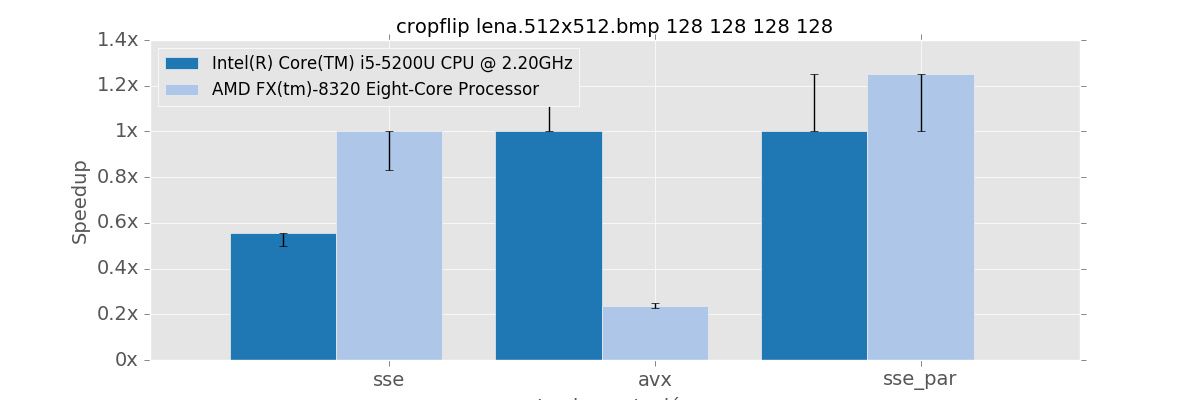
\includegraphics[width=0.65\textwidth]{cropflip-time-speedup} 
\label{fig:cropflip-time-speedup}
\end{figure}

A diferencia de los otros dos filtros, donde el procesamiento de imágenes involucra operaciones aritméticas paralelas, la implementación AVX de	 Cropflip no presenta un 'speedup' tan significativo respecto de las implementaciones de SSE con registros de 128 bits en paralelo \footnote{Los benchmarks en AVX sobre el procesador AMD resultan distorsionados por cuestiones de compatibilidad}. 

\begin{figure}[h]
\centering
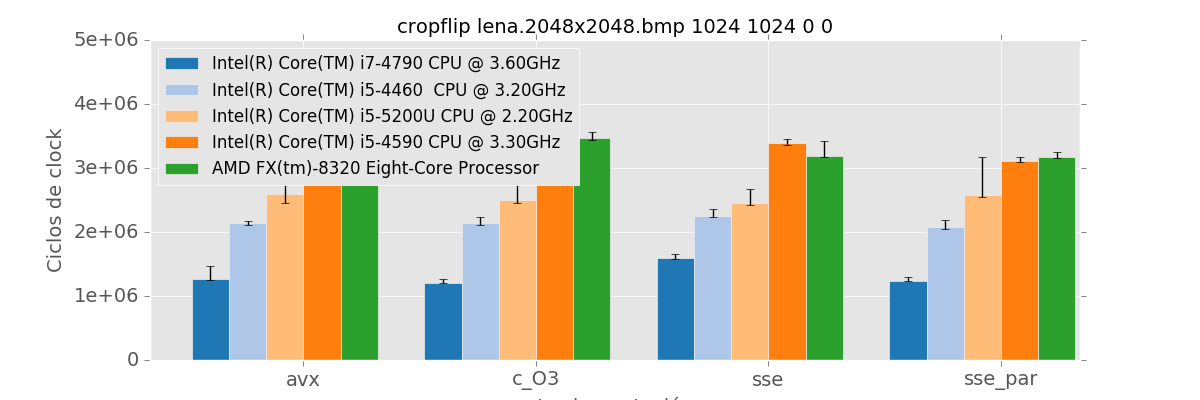
\includegraphics[width=0.65\textwidth]{cropflip-cycles} 
\label{fig:cropflip-cycles}
\end{figure}



Se observa una diferencia de ciclos de clock entre las versiones de SSE a favor del loop unrolling ('SSE Parelo') donde parecería que, aún con buen hitrate, los puntos fuertes  (paralelismo y minimizar branch mispredictions)  no destacan tanto por el hecho de que los accesos a memoria son individuales y no pueden solaparse.
\\
Pudimos corrobar que no es casualidad que el rendimiento de la implementación en C@-O3 sea similar al de las implementaciones SSE (particularmente 'SSE paralelo') utilizando GDB para ver el código compilado y comprobando que vectorizaba con operaciones SSE como se muestra a continuación:

\begin{figure}[h]
\centering
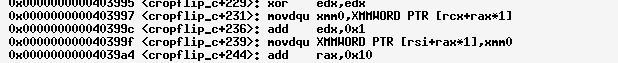
\includegraphics[width=0.65\textwidth]{untitled}
\end{figure}

A modo comparativo también incluímos el análisis de rendimiento entre las diversas optimizaciones para la implementación de C.

\begin{figure}[h]
\centering
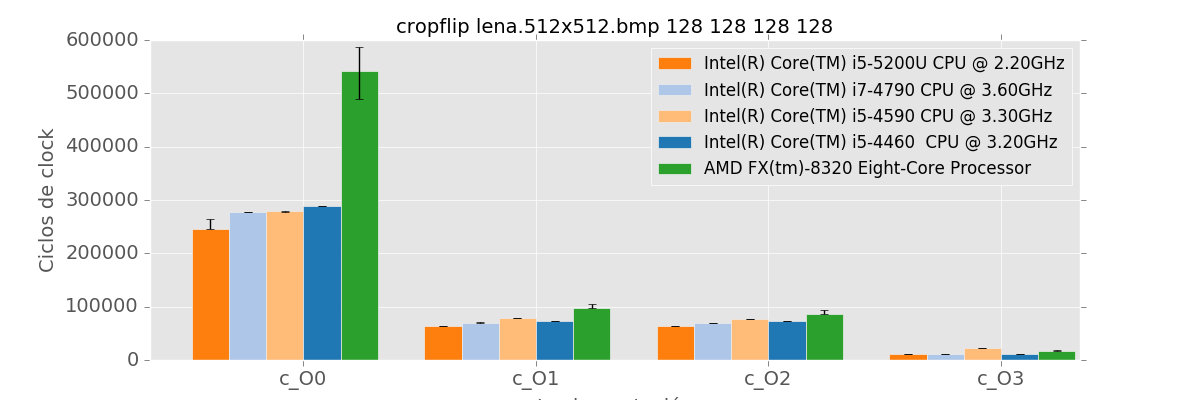
\includegraphics[width=0.65\textwidth]{cropflip-c-cycles} 
\label{fig:cropflip-c-cycles}
\end{figure}

\begin{figure}[h]
\centering
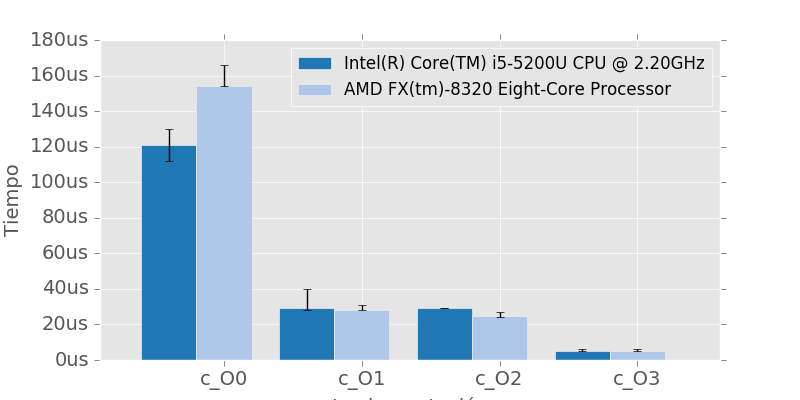
\includegraphics[width=0.65\textwidth]{cropflip-c-time} 
\label{fig:cropflip-c-time}
\end{figure}

\begin{figure}[h]
\centering
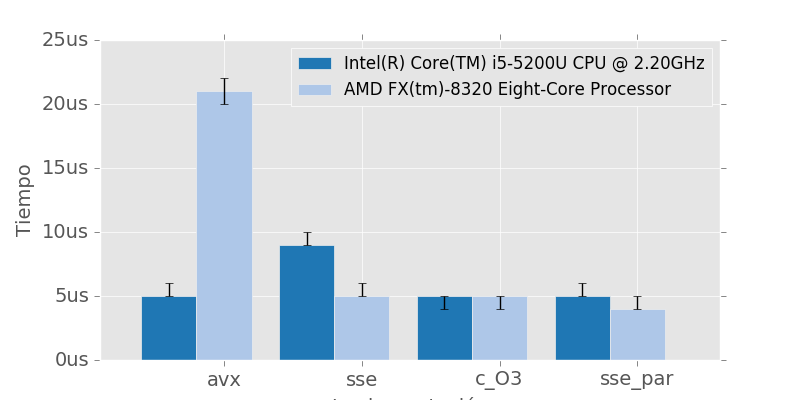
\includegraphics[width=0.65\textwidth]{cropflip-time}
\label{fig:cropflip-time}
\end{figure}

También es remarcable que el salto en rendimiento se produce entre versiones de ASM y de C con optimización menor a -O3, donde bajan del rango de 20-80 a 3-8 microsegundos.

\begin{figure}[h]
\centering
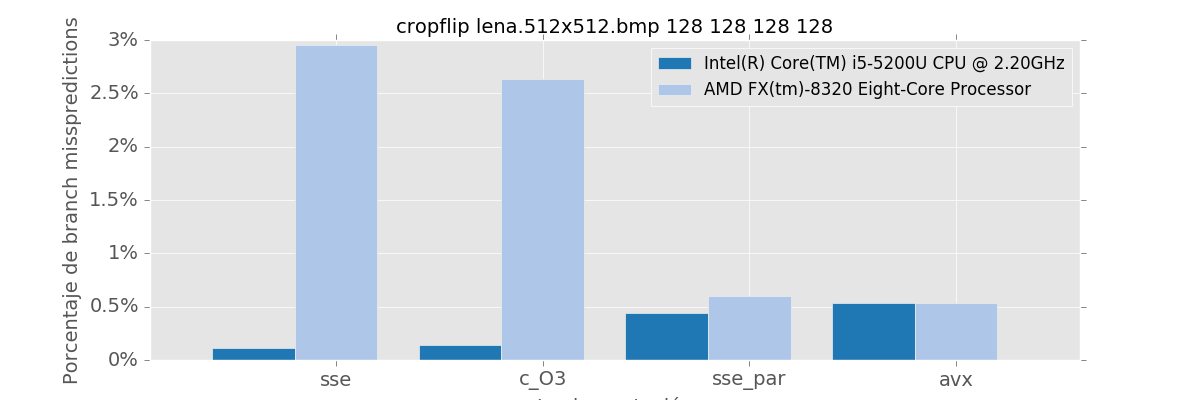
\includegraphics[width=0.65\textwidth]{cropflip-branch-misses}
\label{fig:cropflip-branch-misses}
\end{figure}


En este gráfico se puede apreciar la efectividad del loop unrolling en las implementaciones de AVX y de SSE en paralelo frente a las implementaciones que procesan con un único vector (ya vimos que la implementación en C con optimización O3 también usa un registro XMM para los accesos a memoria).

\begin{figure}[h]
\centering
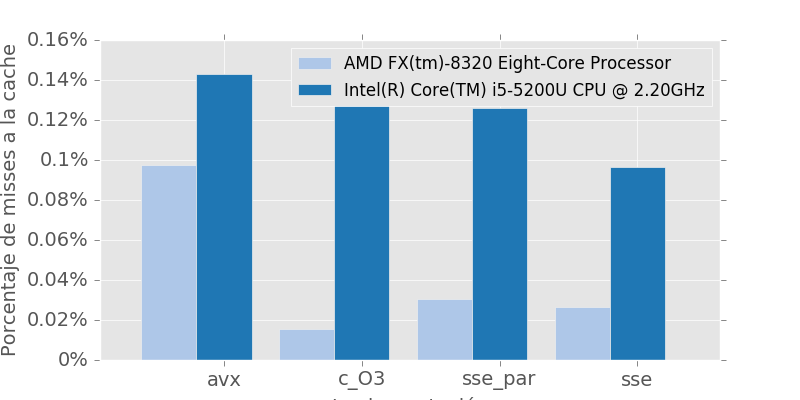
\includegraphics[width=0.65\textwidth]{cropflip-cache-misses}
\label{fig:cropflip-cache-misses}
\end{figure}

Como habíamos anticipado al hablar del loop unrolling en SSE, el tamaño del binario no es lo suficientemente grande como para no poder ser cacheado eficientemente. La vecindad espacial de las tiras de píxeles también colaboran para que el hitrate se mantenga alto aún cuando las filas del crop son contiguas en memoria como comentamos en la descripción.

\begin{figure}[h]
\centering
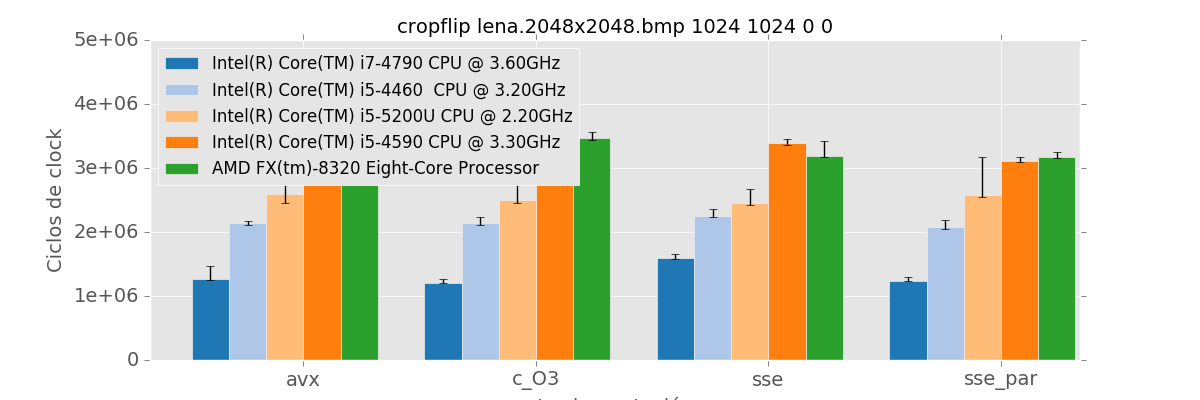
\includegraphics[width=0.85\textwidth]{cropflip-cycles}
\label{fig:cropflip-cycles}
\end{figure}




	
